\section{Implementation}
\label{sec:implementation}

To showcase and benchmark my work, I created an Android app that visualizes sensor data from the device it runs on and also from connected Android Wear devices.
The app is called Sensor Data Logger (\ref{fig:sensorDataLoggerApp}) and can be downloaded for free from the Google Play Store\footnote{\href{https://play.google.com/store/apps/details?id=net.steppschuh.sensordatalogger}{https://play.google.com/store/apps/details?id=net.steppschuh.sensordatalogger}}.

\begin{figure}[H]
	\href{https://github.com/Steppschuh/Sensor-Data-Logger}{
		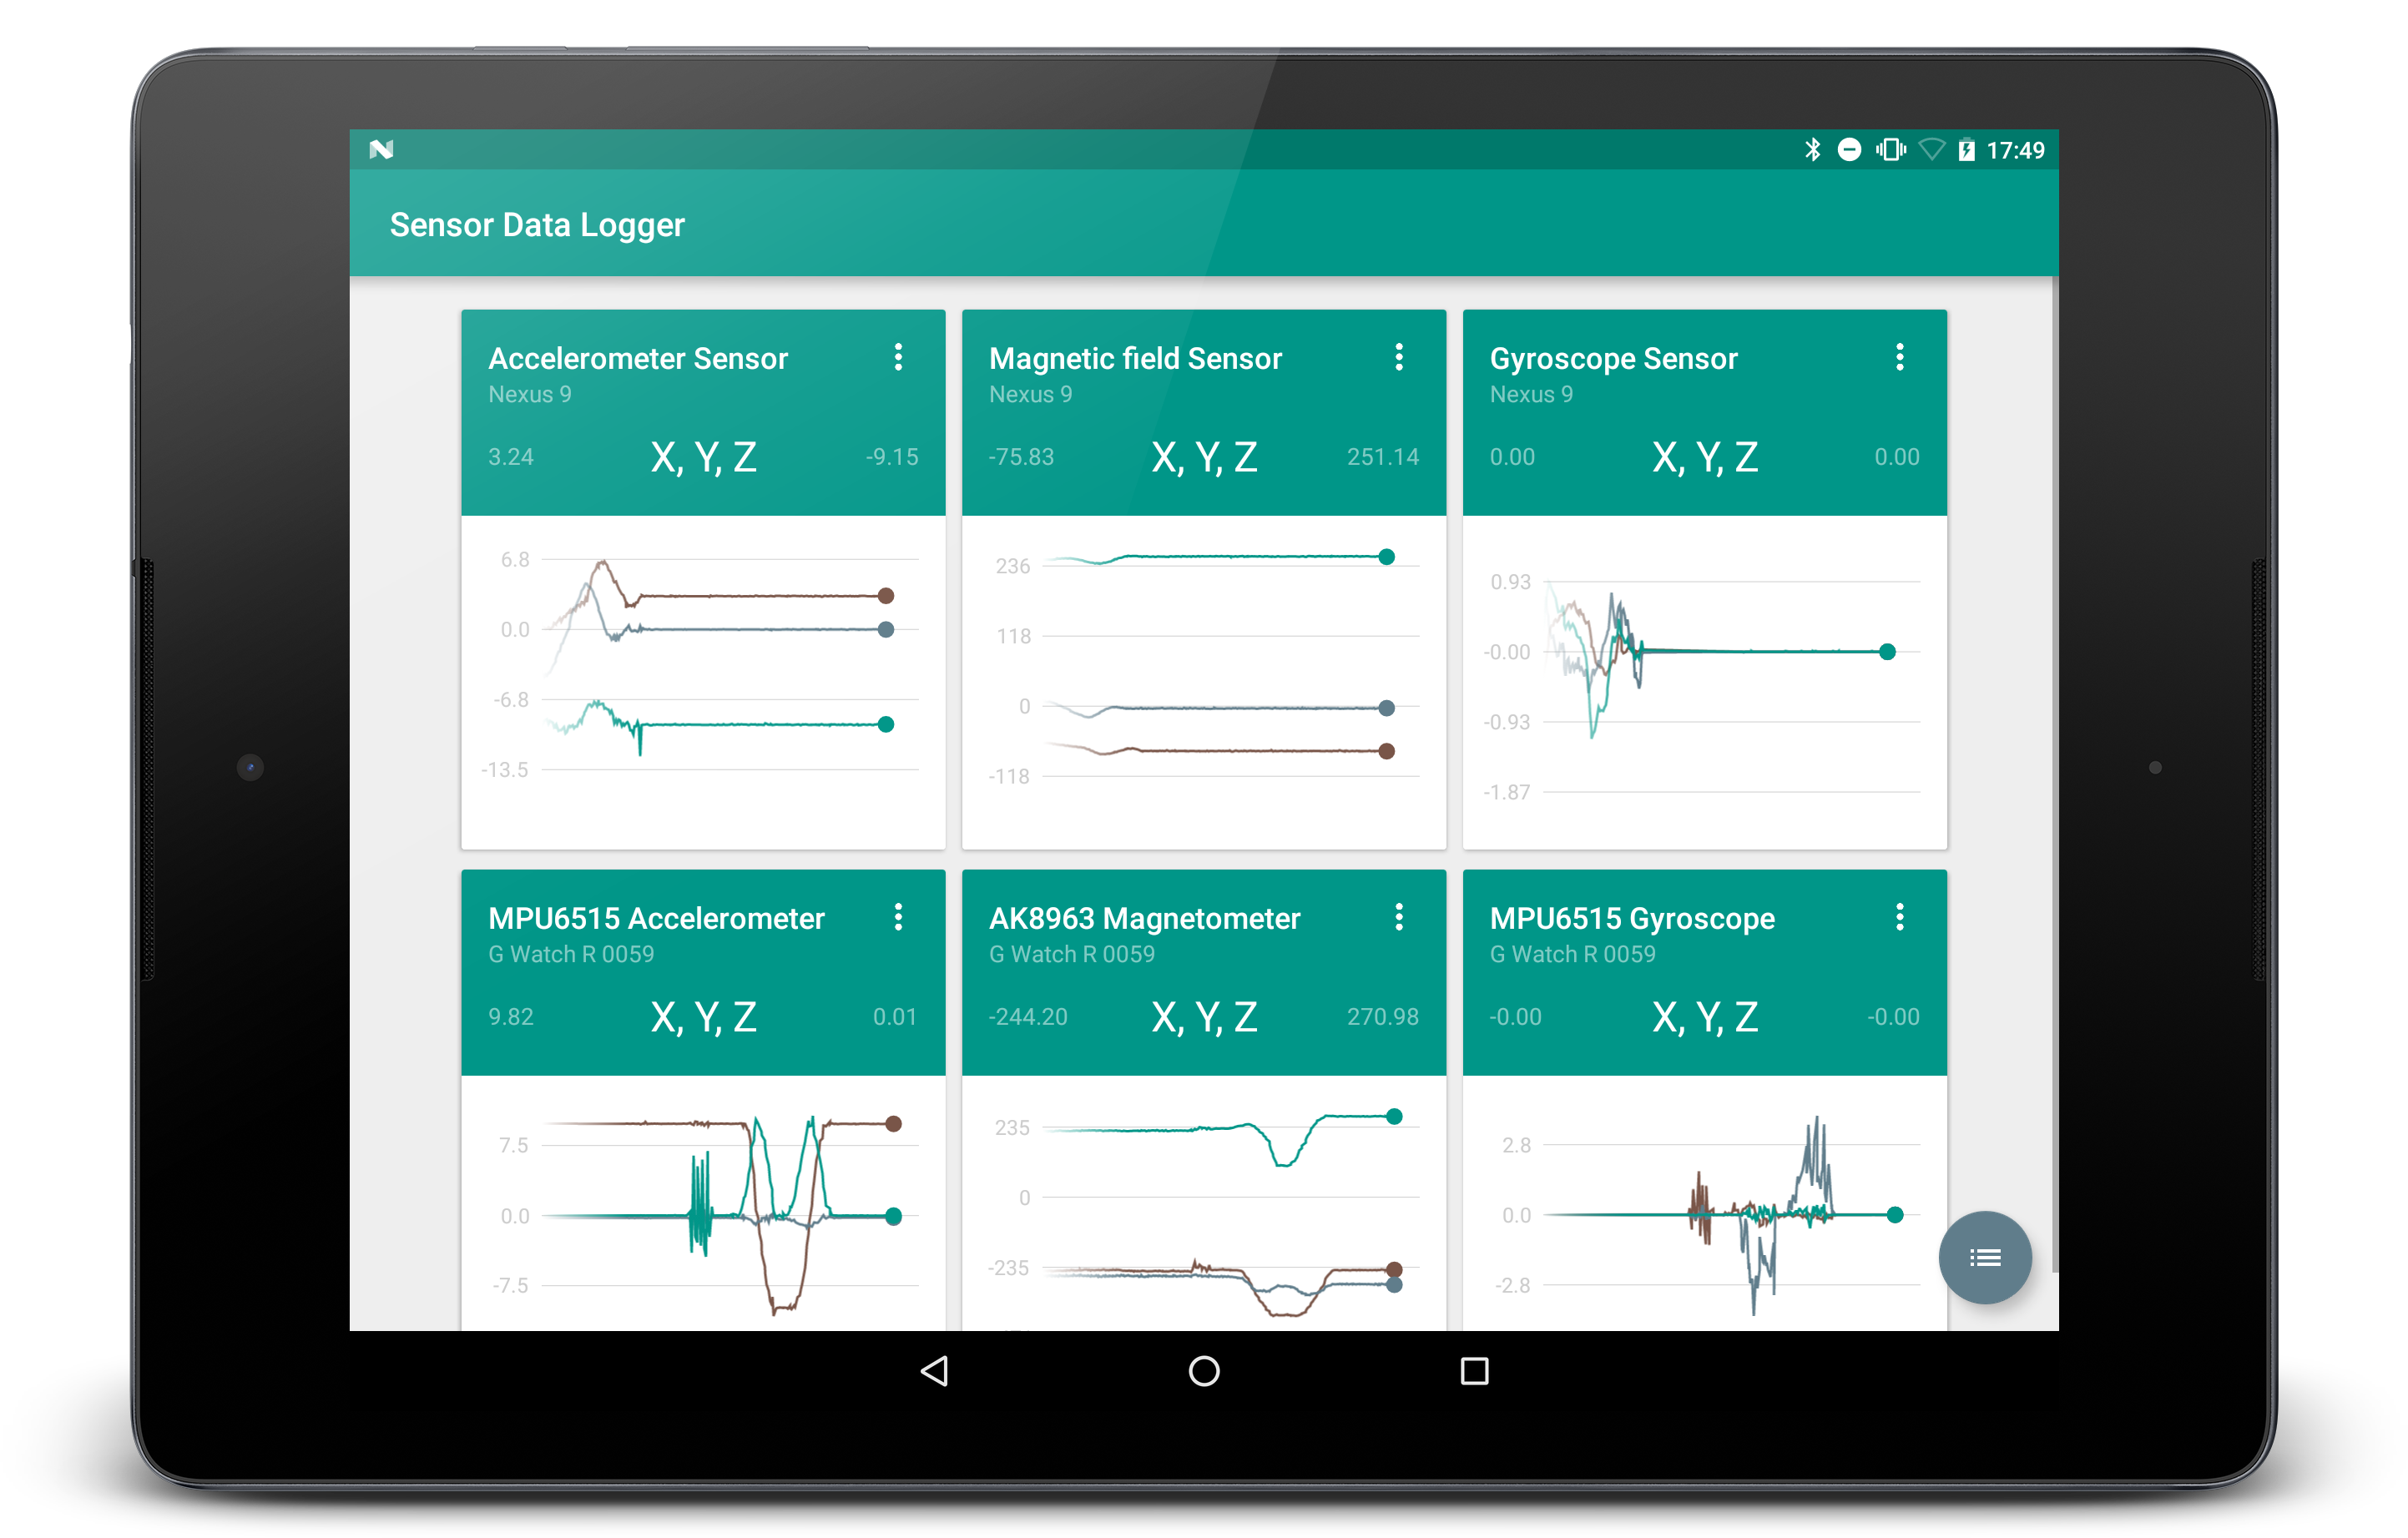
\includegraphics[width=\linewidth]{images/app/charts_landscape_framed.png}
	}
	\caption[Caption for Sensor Data Logger App]{Sensor Data Logger App}
	\label{fig:sensorDataLoggerApp}
\end{figure}

Code samples in the following sections are snippets from this project and can be seen in context in the GitHub repository\footnote{\href{https://github.com/Steppschuh/Sensor-Data-Logger}{https://github.com/Steppschuh/Sensor-Data-Logger}}.

\clearpage

\subsection{Accessing Data}
\label{sec:implementation:accessingdata}

Android provides the |SensorManager|\cite{androiddocs:sensormanager} system service class in order to grant applications access to the device sensors.
The supported sensors can be divided into three categories:

\begin{itemize}[noitemsep]
	\item \textbf{Environmantal sensors} (thermometers, barometers and photometers)
	\item \textbf{Motion sensors} (accelerometers, gyroscopes and gravity sensors)
	\item \textbf{Position sensors} (magnetometers and orientation sensors)
\end{itemize}

Not all sensors are hardware components, the so called ``virtual-'' or ``synthetic sensors'' derive their data from one or more hardware-based sensors.
Examples for these virtual sensors are the linear acceleration sensor, which computes its data based on the accelerometer and the force of gravity.

All sensors can be accessed through the Android sensor framework, which provides classes and interfaces that can be used to figure out which sensors are available on the current device, which capabilities they have and what data they produce.

\subsubsection{Checking Availability}
\label{sec:implementation:checkingavailability}
While most devices have an accelerometer and a magnetometer, only a few have a thermometer.
The availability of sensors can't be guaranteed, it's good practice to check this at runtime:

\begin{lstlisting}[label=getsensormanager]
// get a SensorManager instance
SensorManager sensorManager = (SensorManager) getSystemService(Context.SENSOR_SERVICE);

// get a list of available sensors
List<Sensor> deviceSensors = sensorManager.getSensorList(Sensor.TYPE_ALL);

// check if an accelerometer is available
Sensor accelerometer = sensorManager.getDefaultSensor(Sensor.TYPE_ACCELEROMETER);
if (accelerometer != null) {
	// use accelerometer
} else {
	// perform error handling
}
\end{lstlisting}

If a sensor is available, public methods from the |Sensor|\cite{androiddocs:sensor} class can be used to get detailed information about it.
The name, vendor, version, data range and reporting delay are useful properties, especially because one device can have multiple sensors of the same type.

\subsubsection{Monitoring data changes}
\label{sec:implementation:monitoringdatachanges}
In order to get access to the actual data, a |SensorEventListener|\cite{androiddocs:sensoreventlistener} needs to be registered at the |SensorManager| instance. The |SensorEventListener| is an interface which exposes two callback methods:

\begin{lstlisting}[label=registersensoreventlistener]
// create a new SensorEventListener
SensorEventListener listener = new SensorEventListener() {
	@Override
	public void onSensorChanged(SensorEvent event) {
		// sensor reported new data
	}

	@Override
	public void onAccuracyChanged(Sensor sensor, int accuracy) {
		// sensor accuracy changed
	}
};

// specify a reporting delay for the sensor
int delay = SensorManager.SENSOR_DELAY_NORMAL;

// register the listener for the accelerometer
sensorManager.registerListener(listener, accelerometer, delay);
\end{lstlisting}

The |onSensorChanged| method will be called every time the sensor updates its values. The passed |SensorEvent|\cite{androiddocs:sensorevent} holds the sensor, a timestamp, the accuracy and an array of floats containing the actual values.

If the sensor accuracy changes, which often happens when using location sensors, the |onAccuracyChanged| method will be called.
It can be usefull to care about these accuracies, the location optained from the Cell-ID or Wi-Fi might be more accurate than the latest GPS coordinates for example.
In other cases sensors might need a few seconds to calibrate, like the magnetometer.

When registering a |SensorEventListener|, a delay in microseconds is also passed to the |SensorManager|.
It's worth to notice that this value is more like a suggestion, as other applications and the system can alter it.
Because the reporting delay can impact the battery life of the device, some manufacturers will lower the reporting interval when the device is idle or the display is turned off.

\clearpage

\subsubsection{Monitoring lifecycle changes}
\label{sec:implementation:monitoringlifecyclechanges}
Once a |SensorEventListener| is registered, the system will keep the requested sensor active and continue to report data, even if the user leaves the application.
Hence, one should always unregister listeners as soon as possible in order to prevent battery drain:

\begin{lstlisting}[label=basicactivity]
public class SensorActivity extends Activity implements SensorEventListener {
	private SensorManager sensorManager;
	private Sensor accelerometer;

	@Override
	public final void onCreate(Bundle savedInstanceState) {
		super.onCreate(savedInstanceState);
		setContentView(R.layout.main);
		sensorManager = (SensorManager) getSystemService(Context.SENSOR_SERVICE);
		accelerometer = sensorManager.getDefaultSensor(Sensor.TYPE_ACCELEROMETER);
	}

	@Override
	protected void onResume() {
		super.onResume();
		sensorManager.registerListener(this, accelerometer, SensorManager.SENSOR_DELAY_NORMAL);
	}

	@Override
	protected void onPause() {
		super.onPause();
		sensorManager.unregisterListener(this);
	}

	@Override
	public final void onSensorChanged(SensorEvent event) {
		StringBuilder log = new StringBuilder("Acceleration:");
		log.append(" X: ").append(String.valueOf(event.values[0]));
		log.append(" Y: ").append(String.valueOf(event.values[1]));
		log.append(" Z: ").append(String.valueOf(event.values[2]));
		System.out.println(log.toString());
	}

	@Override
	public final void onAccuracyChanged(Sensor sensor, int accuracy) {
		// sensor accuracy changed
	}
}
\end{lstlisting}

This very basic example activity would print accelerometer data to the console once deployed.
Keep in mind that it lacks exception handling, as mentioned in \ref{sec:implementation:checkingavailability}.
I presume a basic understanding of how the Android activity\cite{androiddocs:activity} lifecycle works.

\subsection{Persisting Data}
Once a sensor is reporting data, a new |SensorEvent| will be passed to the callback every few milliseconds.
The |values| float array will contain new data, however the system won't allocate a new object for every update in order to improve performance.
Handling these values without knowing about its object identity might cause confusion, as they will be overwritten with every update.
To prevent this, a new float array can be used to hold the event data:

\begin{lstlisting}[label=arraycopy]
@Override
public void onSensorChanged(SensorEvent event) {
	// create a new float array with the same size
	float[] values = new float[event.values.length];

	// copy data from event values
	System.arraycopy(event.values, 0, values, 0, event.values.length);

	// persist values in some way
	persistValues(values);
}
\end{lstlisting}

For my project, I needed to look back at sensor events from the past few seconds in order to detect patterns and to extract features.
I created some helper classes\cite{sensordatalogger:datapackage} that allowed me to wrap sensor event data in POJOs\footnote{Plain old Java objects}, this way they could be persisted in a batch-like structure.

There is a |Data|\cite{sensordatalogger:data} class which can wrap the values of a |SensorEvent|, its source and a timestamp.
This is necessary because the |SensorEvent| holds references to objects that aren't required multiple times and because there's no public constructor available.

The |DataBatch|\cite{sensordatalogger:databatch} class holds and manages a list of |Data| objects.
It has a customizable capacity, one can add or remove |Data| and it will automatically remove old |Data| if the capacity has been reached.
It also provides some convenience methods, for example to get |Data| from within a given time range.

\begin{lstlisting}[label=datahelperclasses]
private Map<Integer, DataBatch> sensorDataBatches = new HashMap<>();

@Override
public void onSensorChanged(SensorEvent event) {
	float[] values = new float[event.values.length];
	System.arraycopy(event.values, 0, values, 0, event.values.length);

	// create a new Data object
	Data data = new Data(values);

	// get a previously initialized DataBatch
	DataBatch dataBatch = getDataBatch(event.sensor.getType());

	// add the new data
	dataBatch.addData(data);
}

public DataBatch getDataBatch(int sensorType) {
	DataBatch dataBatch = sensorDataBatches.get(sensorType);
	if (dataBatch == null) {
		dataBatch = new DataBatch(sensorType);
		sensorDataBatches.put(sensorType, dataBatch);
	}
	return dataBatch;
}
\end{lstlisting}

This code would fill up a |DataBatch| with event data for each requested sensor type.
The batches are serializable and come in handy when writing data into a file or transferring it to another device.

\subsection{Transferring Data}
Actually using the sensor event data requires transferring it to a device with sufficient processing power.

\subsubsection{General Approach}
In a world where the IoT\footnote{Internet of Things} is a big topic, data is usually uploaded to the cloud and processed on powerfull servers.
Although one could do that from a mobile device, this approach would produce a huge amount of traffic and ultimately lead to privacy concerns.

The setup that this work is about could be seen as a peer to peer network between a mobile device and multiple wearables.
Because the devices are connected with each other, there's no need to detour data through the internet.
By default, wearables are connected via Bluetooth with a mobile device.
On the Android platform, this connection can be accessed through the |WearableApi|\cite{androiddocs:wearable}.

\subsubsection{The Wearable Data Layer}
The Data Layer API is part of of the Google Play Services (version 5+) and can be reached using an instance of the |GoogleApiClient|\cite{androiddocs:googleapiclient}.
Because some Play Services may not be available on every device, the |GoogleApiClient| needs to be setup first:

\begin{lstlisting}[label=googleapiclient]
GoogleApiClient googleApiClient = new GoogleApiClient.Builder(context)
		.addConnectionCallbacks(new ConnectionCallbacks() {
			@Override
			public void onConnected(Bundle connectionHint) {
				// start using the Data Layer API
			}
			@Override
			public void onConnectionSuspended(int cause) {
				// something interrupted the connection
			}
		})
		.addOnConnectionFailedListener(new OnConnectionFailedListener() {
			@Override
			public void onConnectionFailed(ConnectionResult result) {
				// API might not be available
			}
		})
		.addApi(Wearable.API)
		.build();
\end{lstlisting}

asdf

\begin{itemize}[noitemsep]
	\item What to transfer
		\begin{itemize}
			\item suitable data types
			\item serialization
		\end{itemize}
	\item How to transfer
		\begin{itemize}
			\item Available APIs and Protocols
			\item Pros and cons of different methods
		\end{itemize}
\end{itemize}
\lipsum[1]
\lipsum[2]
\lipsum[3]
\lipsum[4]
\lipsum[5]
\lipsum[1]
\lipsum[2]
\lipsum[3]
\lipsum[4]
\lipsum[5]
\lipsum[2]
\lipsum[3]
\lipsum[4]
\lipsum[5]


\clearpage